% 本文件是示例论文的一部分
% 论文的主文件位于上级目录的 `main.tex`
\chapter{检测系统的设计与实现}

\section{需求分析}
该系统需要为用户提供两个模块的功能,一个是头盔佩戴情况检测功能,一个是历史检测数据查询功能,本文为这两个功能各自设计并实现了前端页面。检测页面允许用户上传待检测图片或视频,并需要支持用户自定义检测模型、IoU和置信度参数。检测完成之后,需要将带有目标边界框的结果图片返回给前端并展示在页面上,供用户查看。查询页面可供用户查询历史检测记录,允许用户对驾驶员、检测时间、检测地点等字段进行过滤。检测结果要以可视化的形式展现出来,方便用户进行数据分析。

\section{系统整体架构}
\begin{figure}[!htb]
    \centering
    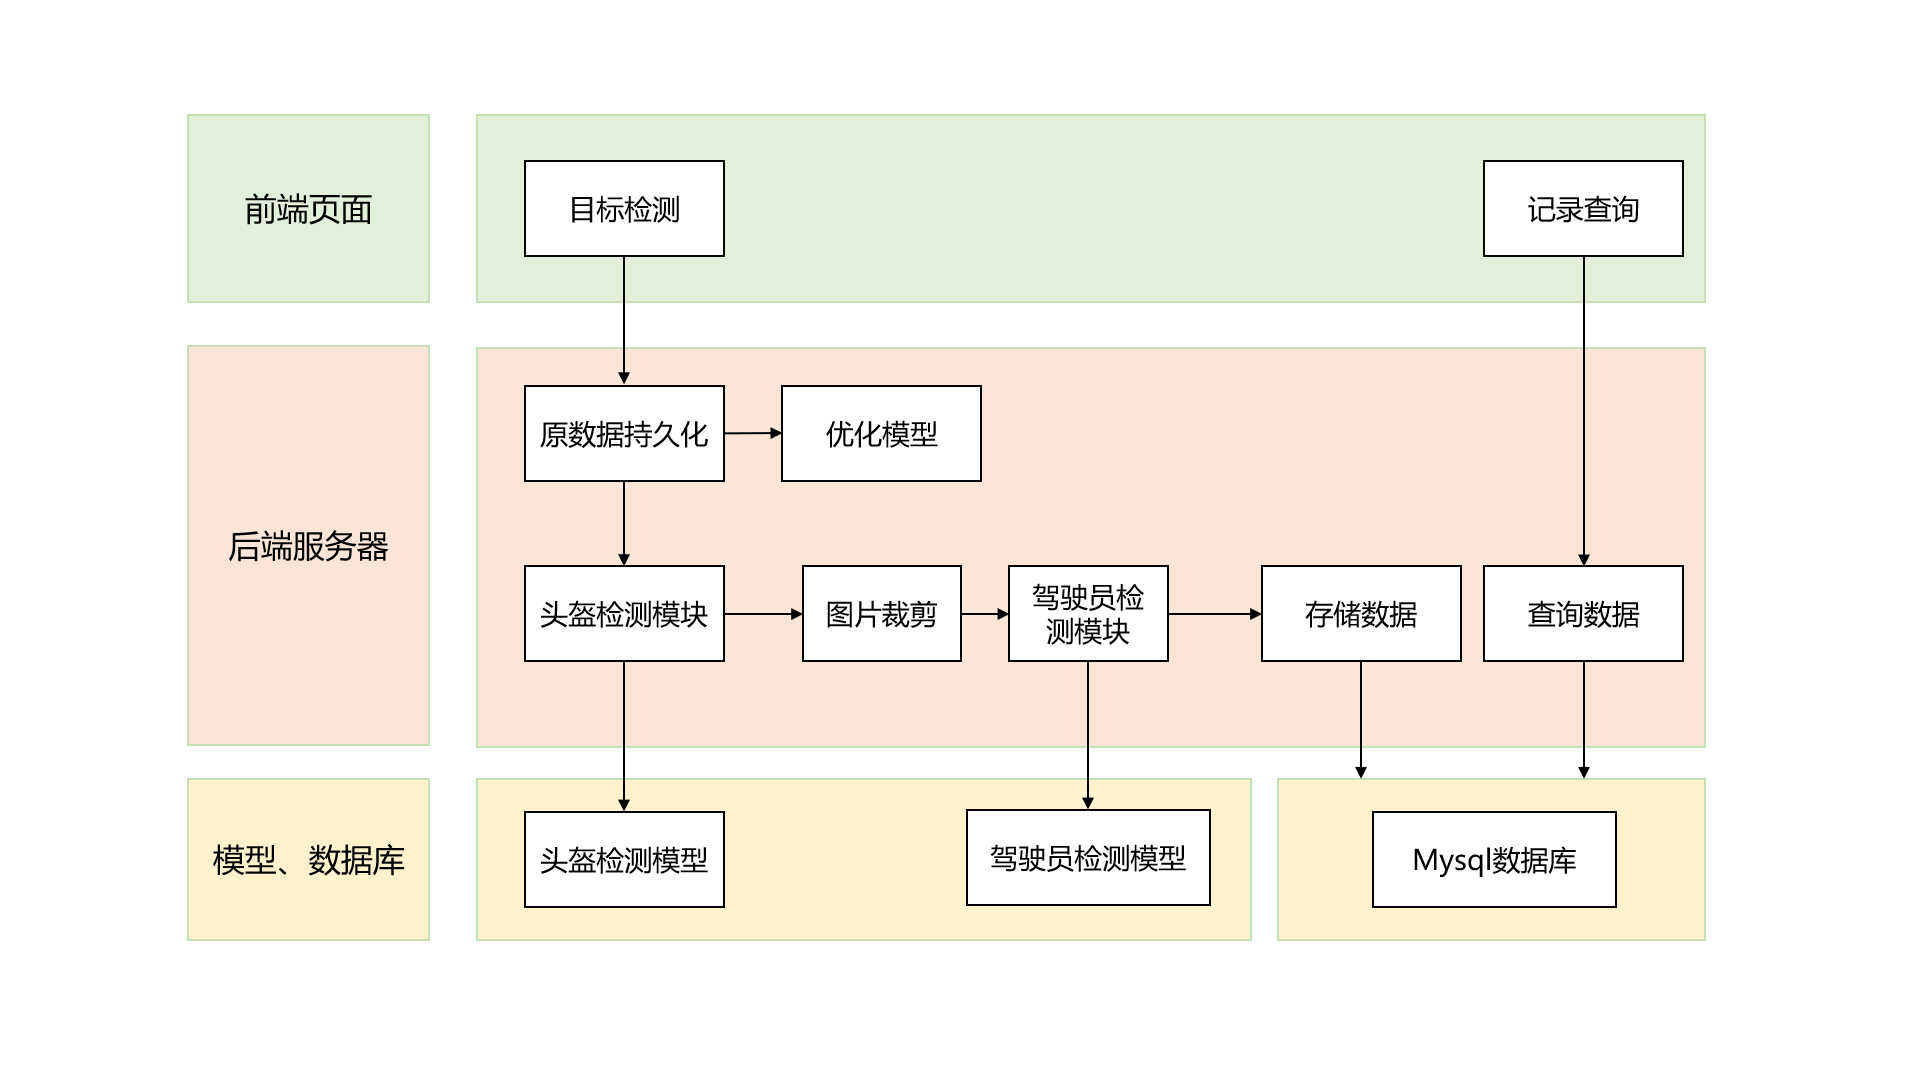
\includegraphics[width=1\textwidth]{figs/chap05/struct.png}
    \caption{系统架构图}
    \label{fig:struct}
\end{figure}
本系统整体架构如\ref{fig:struct}所示。前端为用户提供目标检测和记录查询两个功能,后端负责实现前端的这两个请求接口。后端在处理用户的目标检测请求时,首先会将用户输入的原数据做持久化,后续可以将这些数据作为新的数据集,不断优化模型。然后后端会把用户传入的自定义检测模型、IoU以及置信度参数动态拼接到python脚本里,调用已经训练好的头盔佩戴检测模型进行预测。在python脚本里,设置predict参数save\_crop=True,会在预测之后根据目标检测框对原数据进行裁剪。后端会对这些裁剪之后的图片作为驾驶员检测模型的输入,进一步检测每一位驾驶员的信息。两步检测完成后,将检测结果,包括驾驶员、头盔佩戴情况、检测时间等信息保存到Mysql数据库。最后将带有目标检测框的检测结果返回给前端,展示给用户。

用户请求记录查询接口时,前端将驾驶人、检测时间等参数传给后端,后端根据过滤条件去数据库查询历史数据。前端在这里通过ECharts组件实现了数据的可视化,将检测结果以柱状图、折线图和饼图的方式展示。


\section{前端模块设计与实现}
前端界面分为目标检测界面和记录查询界面。两个界面都以灰、蓝色为主题色调,并且背景以及各个功能区的CSS样式几乎一样,使得两个页面非常协调。
\subsection{目标检测界面}
\subsubsection{界面布局}
目标检测界面的布局如\ref{fig:detAll}所示。该界面包括显示区、参数设置区、系统消息区、功能触发区以及菜单。

\begin{figure}[!htb]
    \centering
    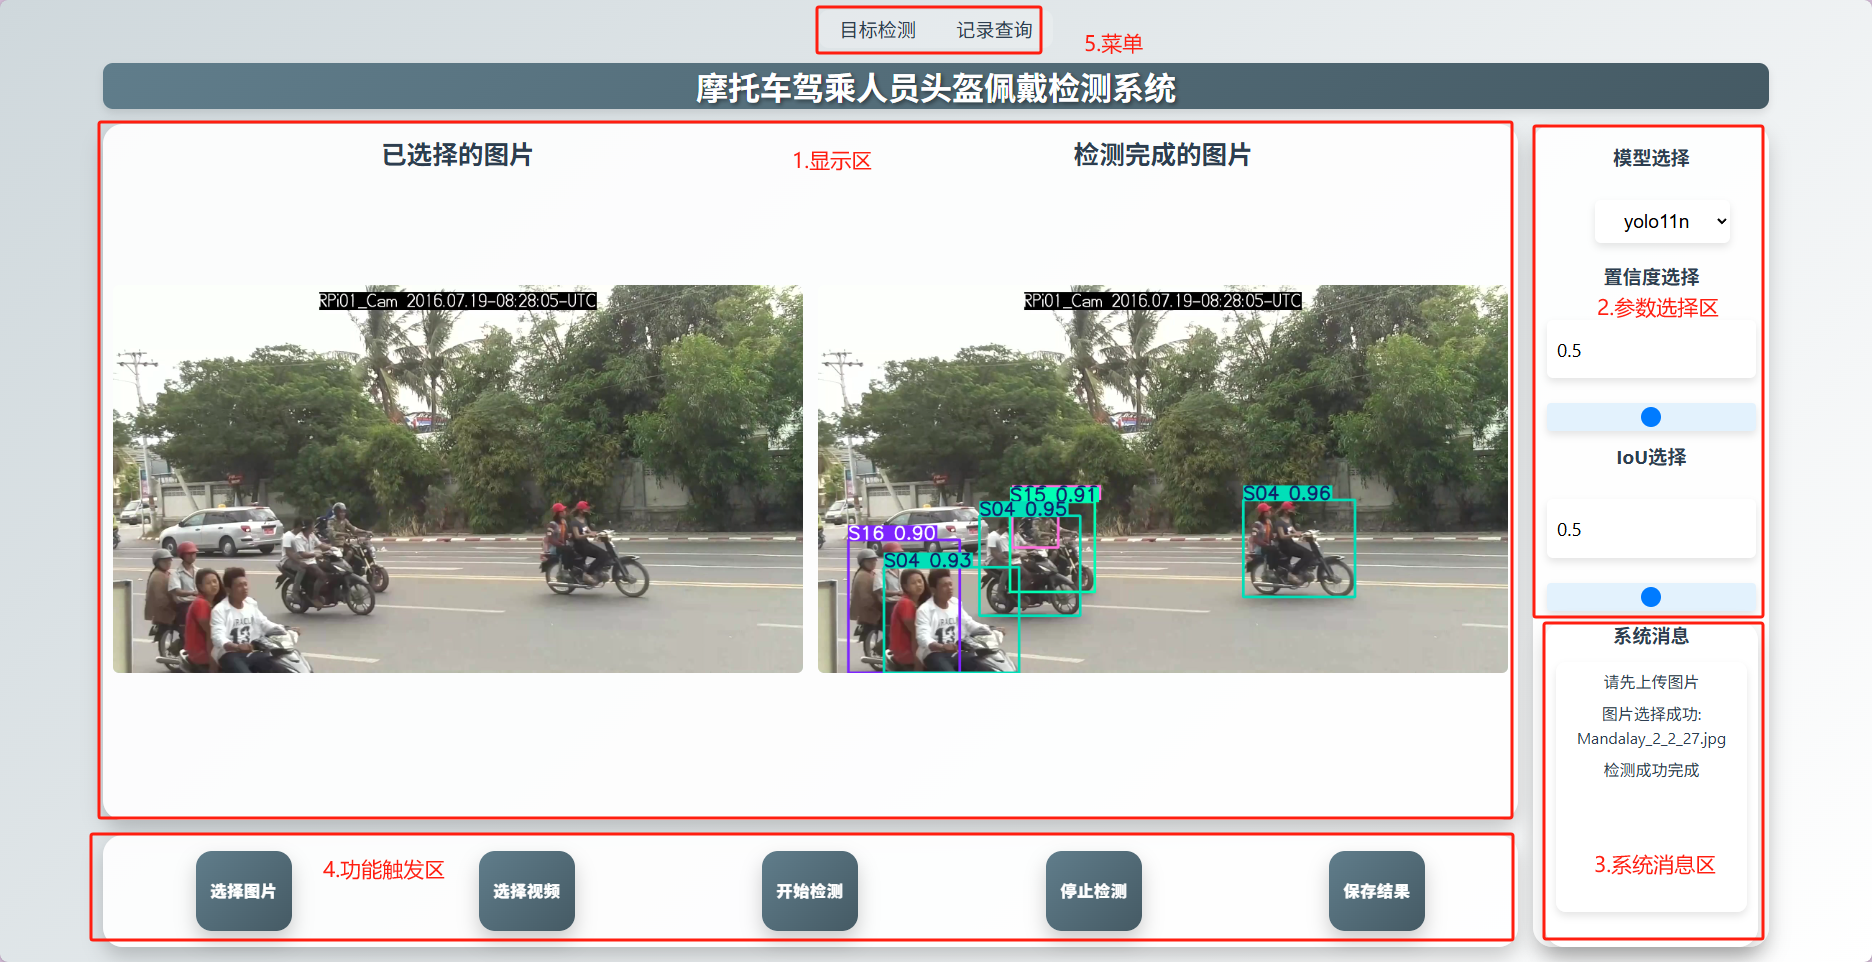
\includegraphics[width=0.9\textwidth]{figs/chap05/detAll.png}
    \caption{目标检测界面布局}
    \label{fig:detAll}
\end{figure}

显示区是页面中最大,最主要的区域,用于展示用户上传的原数据,以及检测结果。该区域被设置为flex布局,左右两边的图像在整个显示区是左右对称的,且大小相同。右侧参数设置区允许用户调整检测模型、Iou和置信度。右下方的系统消息区用来展示用户每一步的操作情况。下方的功能触发区给用户提供选择图片和视频、请求检测、终止当前检测以及保存检测结果的功能。最上方的菜单用于切换检测界面和查询界面。

\subsubsection{功能测试}
首先对检测界面的参数设置区进行检测。对同一张图片,设置不同置信度参数。\ref{fig:conf1}和\ref{fig:conf2}分别展示了置信度设置为0.5和0.95时的检测情况。结果表明,当置信度从0.5调整为0.95后,模型漏检了三个目标。通过查看后台python脚本执行日志,用户能够选择不同的模型进行目标检测。

\begin{figure}[!htb]
    \centering
    \begin{minipage}{0.45\textwidth} % 调整宽度以适应需求,两张图总宽度接近1
        \centering
        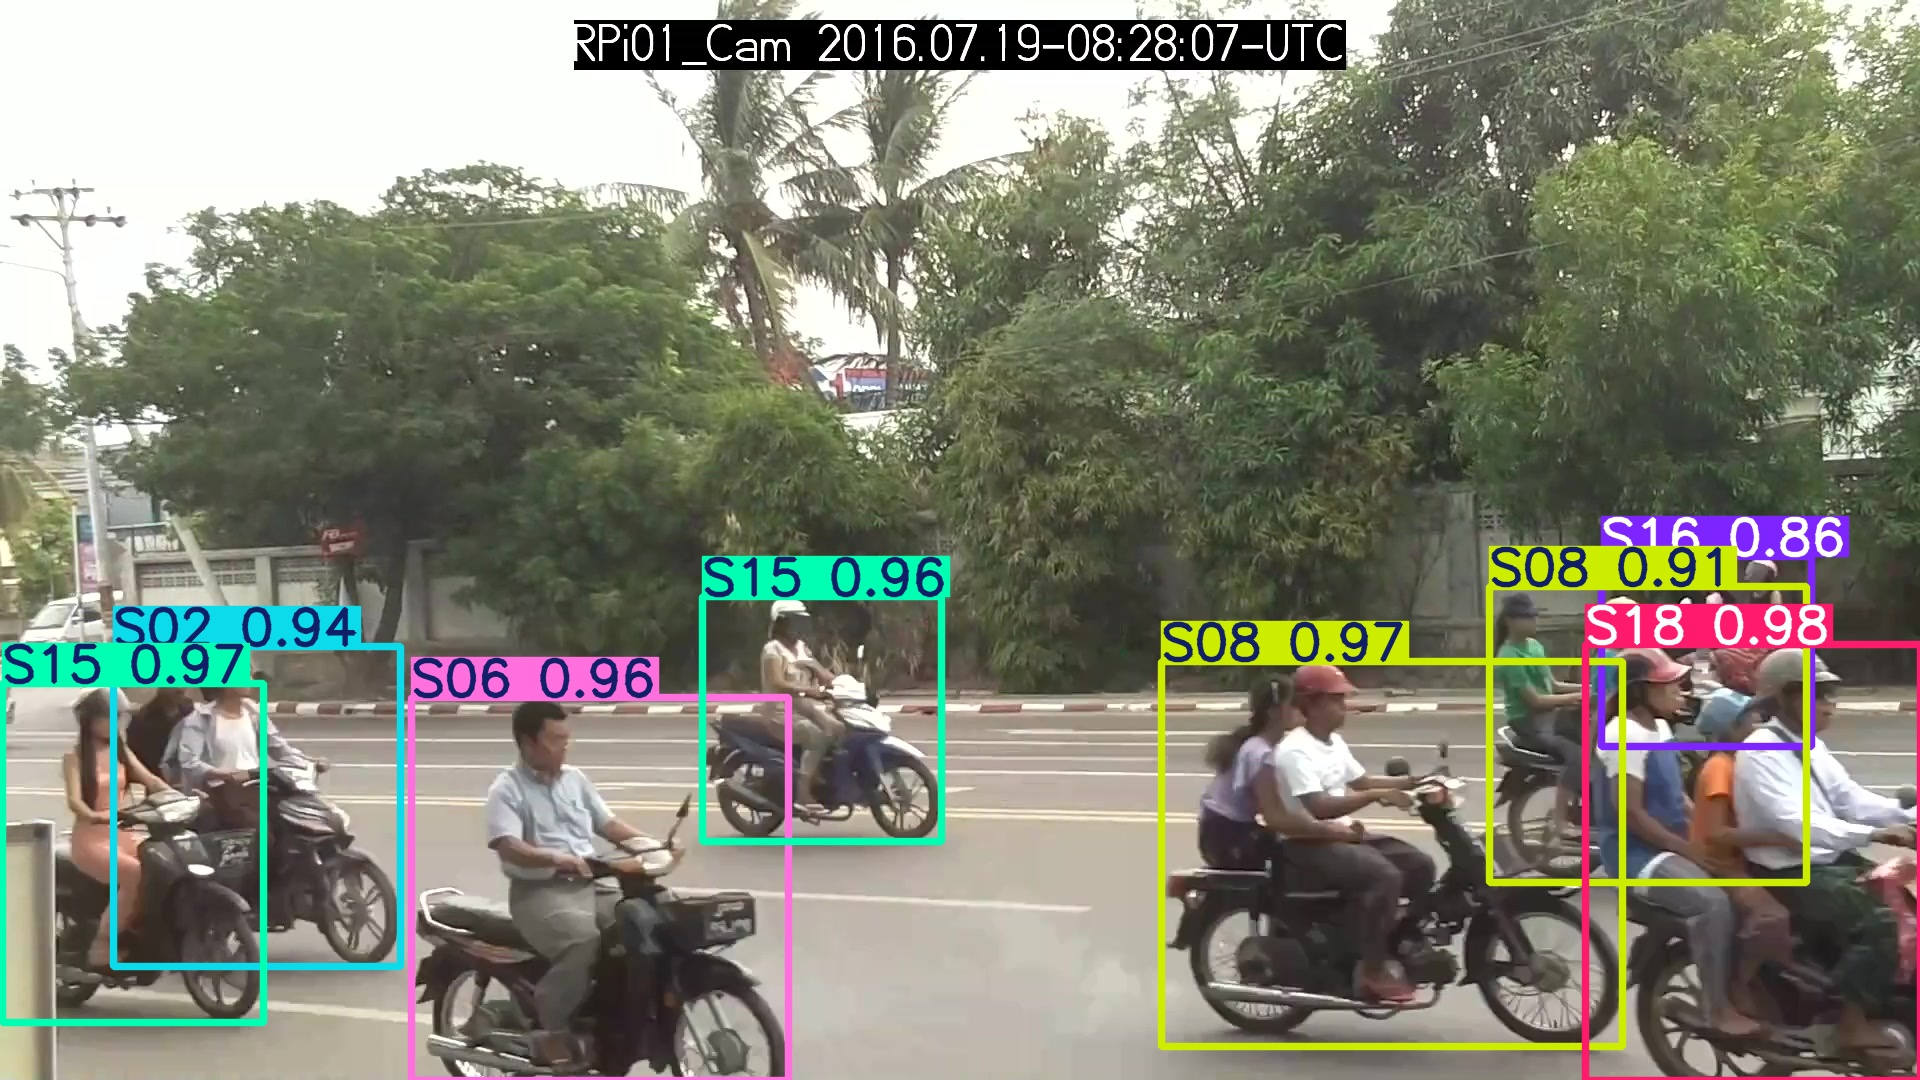
\includegraphics[width=\textwidth]{figs/chap05/conf1.jpg}
        \caption{置信度0.5}
        \label{fig:conf1}
    \end{minipage}
    \hfill % 使两张图片之间保持一定距离
    \begin{minipage}{0.45\textwidth}
        \centering
        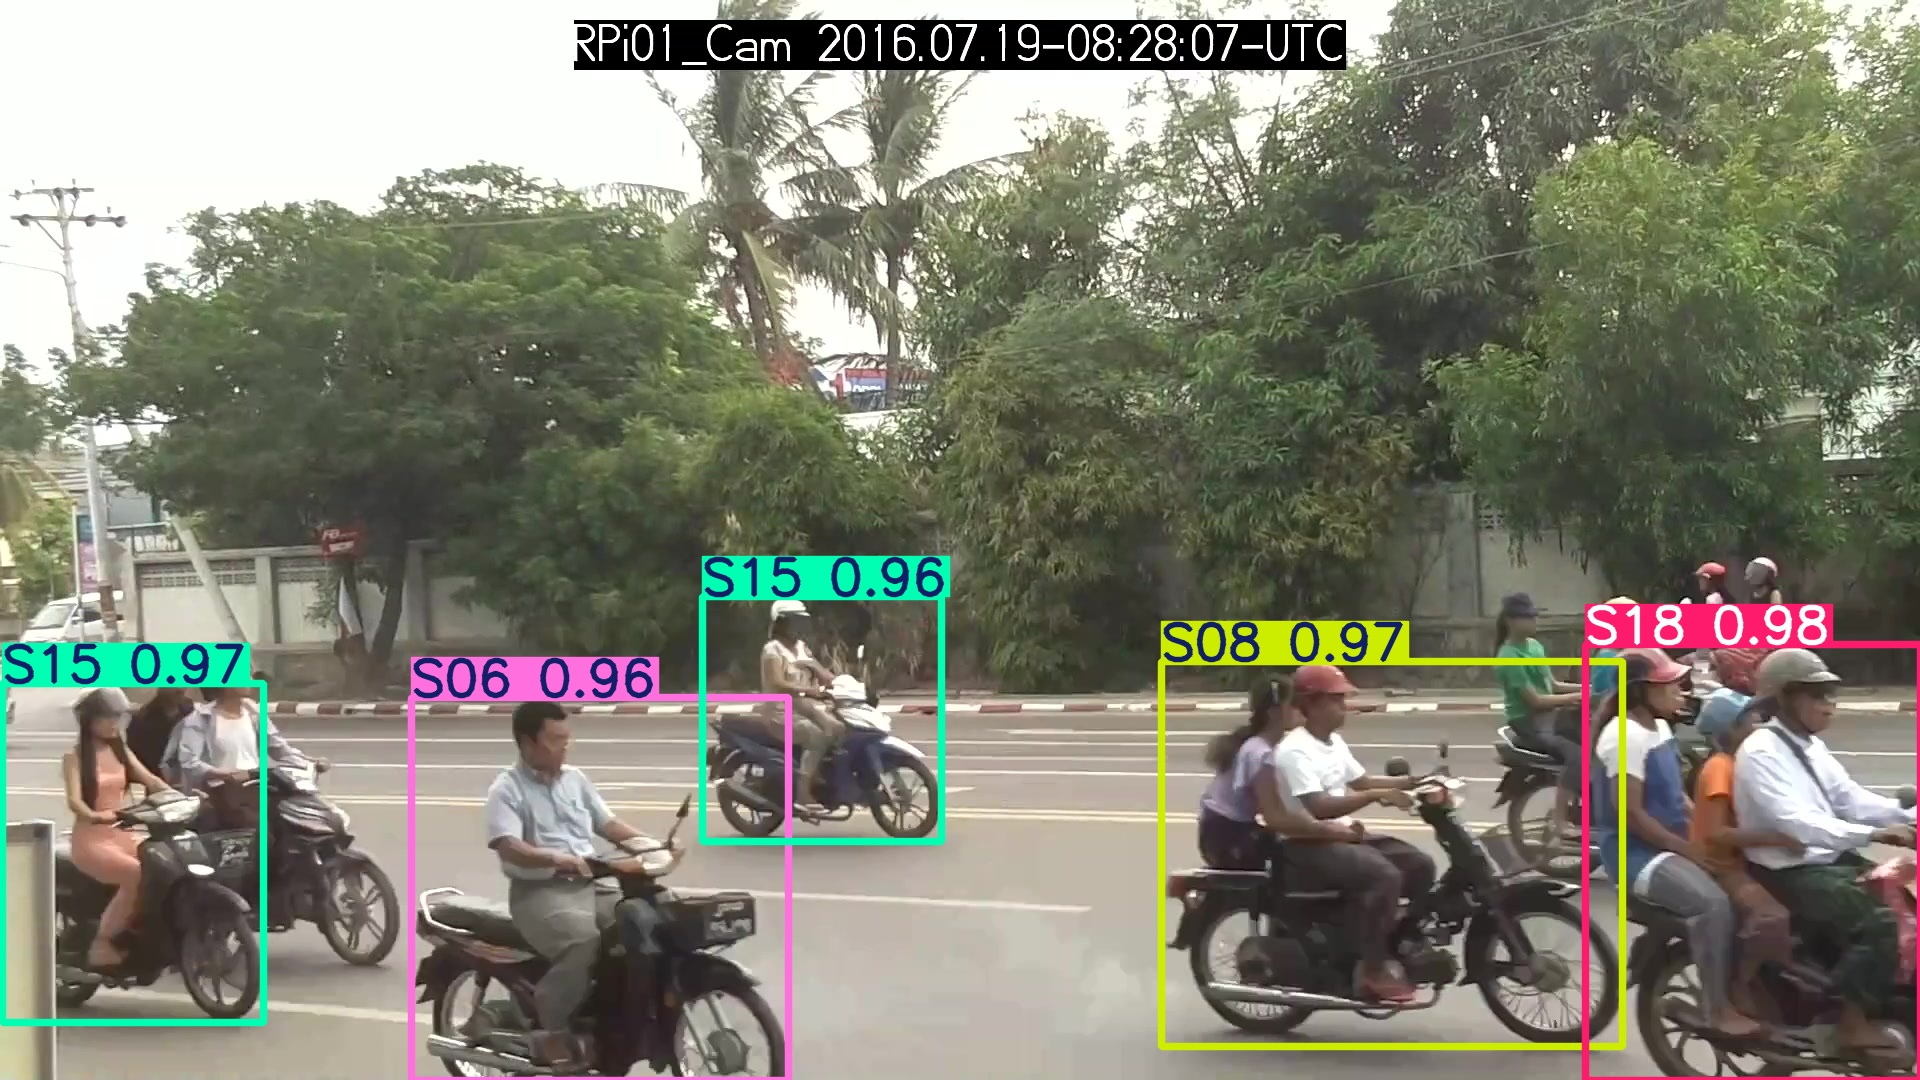
\includegraphics[width=\textwidth]{figs/chap05/conf2.jpg}
        \caption{置信度0.95}
        \label{fig:conf2}
    \end{minipage}
  \end{figure}

然后对下方的功能触发区进行测试。该系统除了图片之外,还支持用户上传视频进行检测。经测试,上传视频并进行检测的功能可以正常使用,效果如\ref{fig:video}所示。且用户点击保存结果后,会触发浏览器的下载功能,将检测结果保存到本地。在整个测试过程中,系统消息区可以将用户的操作结果正确展示出来。

\begin{figure}[!htb]
    \centering
    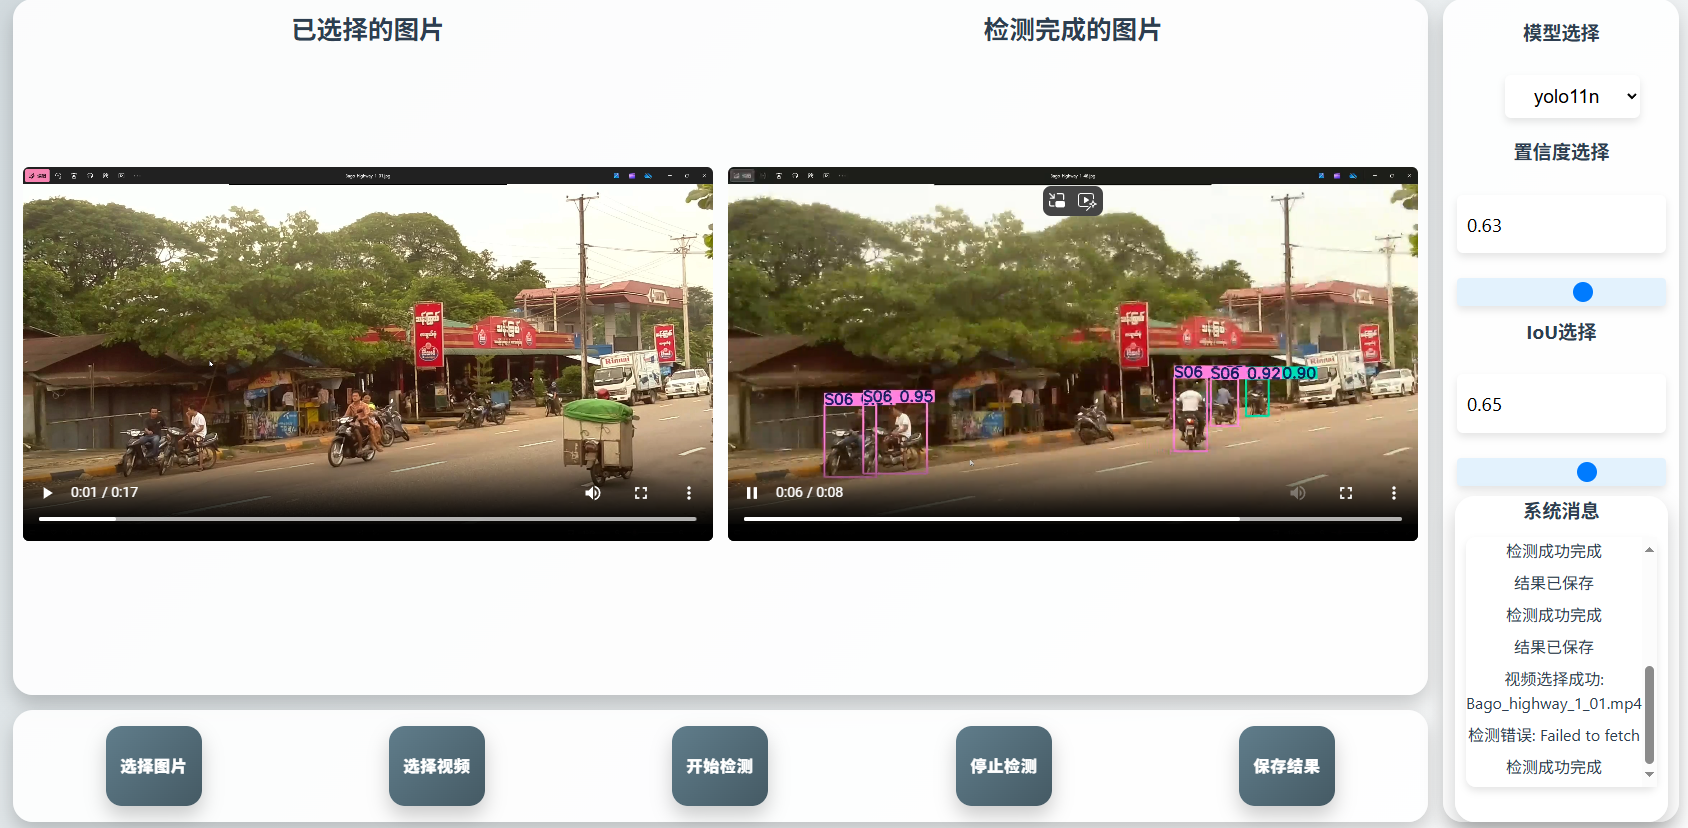
\includegraphics[width=0.9\textwidth]{figs/chap05/video.png}
    \caption{视频检测测试}
    \label{fig:video}
\end{figure}

\subsection{记录查询界面}
\subsubsection{界面布局}
记录查询界面布局见\ref{fig:search}。该界面为用户提供了记录查询功能,用户可以设置过滤条件,对历史记录进行查询。下方是查询结果的展示区域,这里提供了柱状图、折线图和饼图三种可视化方式。

\begin{figure}[!htb]
    \centering
    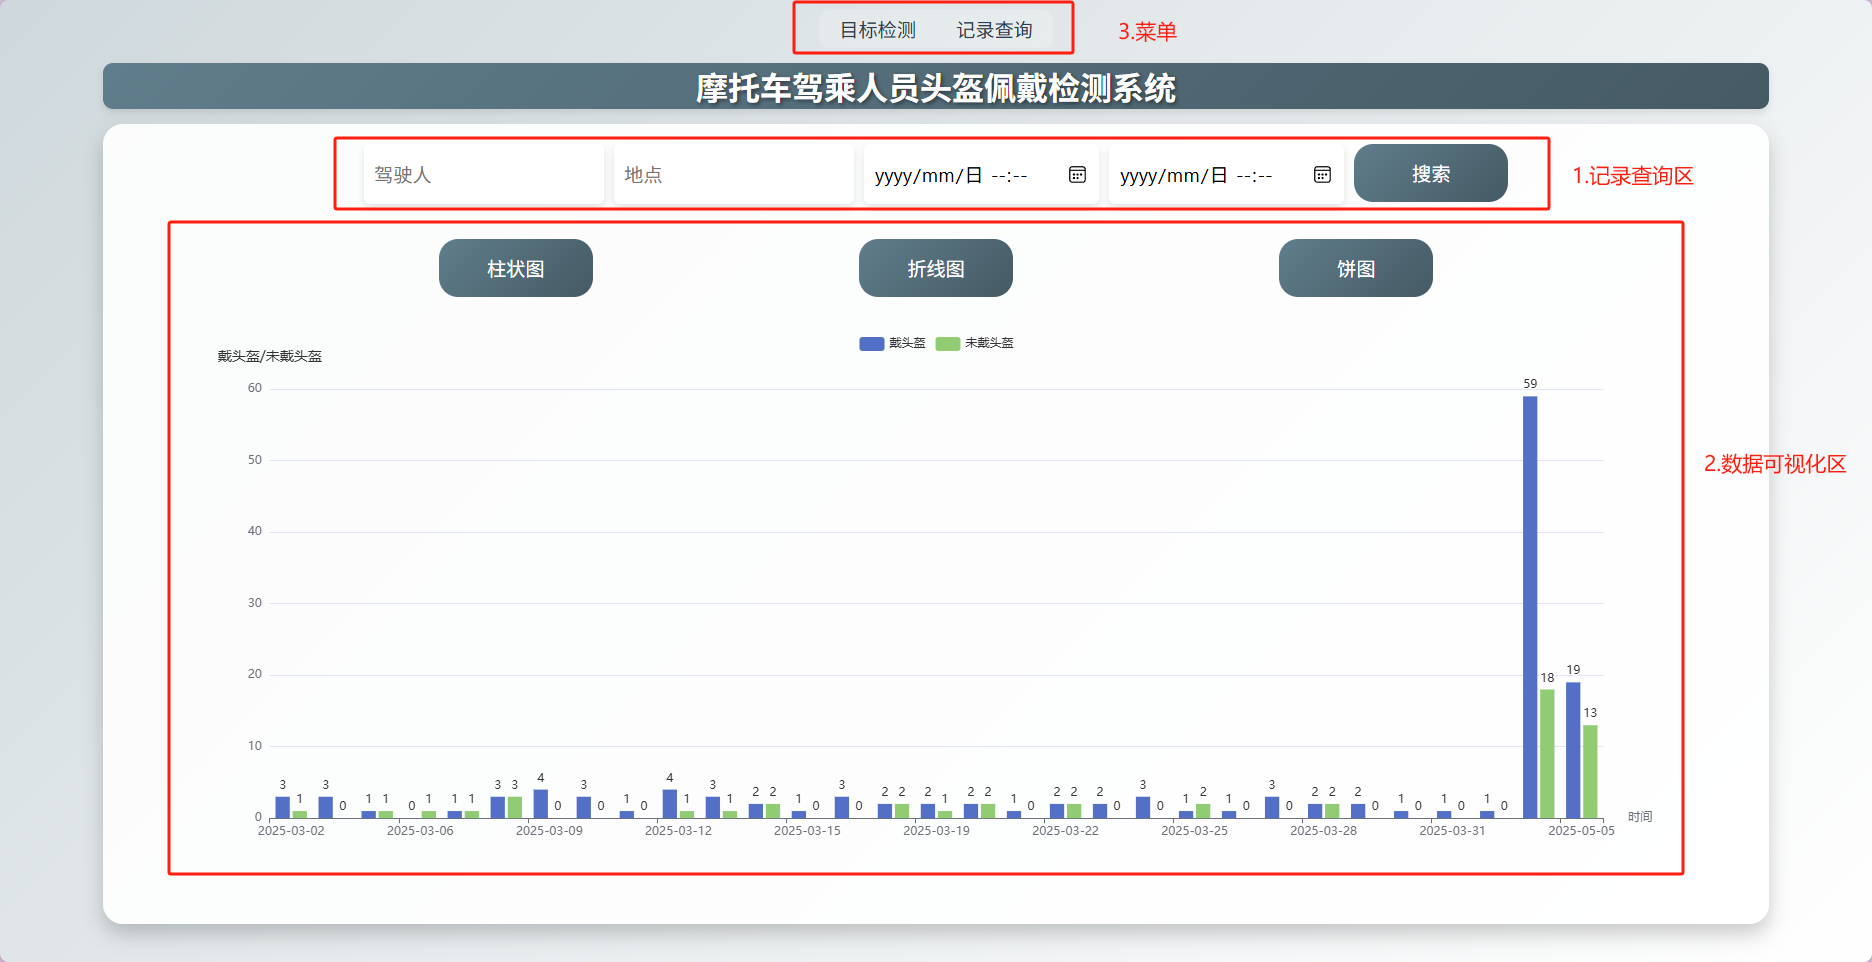
\includegraphics[width=0.9\textwidth]{figs/chap05/search.png}
    \caption{目标检测界面布局}
    \label{fig:search}
\end{figure}

\subsubsection{功能测试}
对记录查询功能进行测试,设置为查询3月21日到5月5日的数据,可以通过下方的柱状图看出,过滤条件是生效的。切换不同的可视化图标,都可以展示正确结果。测试结果如\ref{fig:data1},\ref{fig:data2},\ref{fig:data3}。

\begin{figure}[!htb]
    \centering
    \begin{minipage}{0.3\textwidth} % 调整宽度以适应需求,两张图总宽度接近1
        \centering
        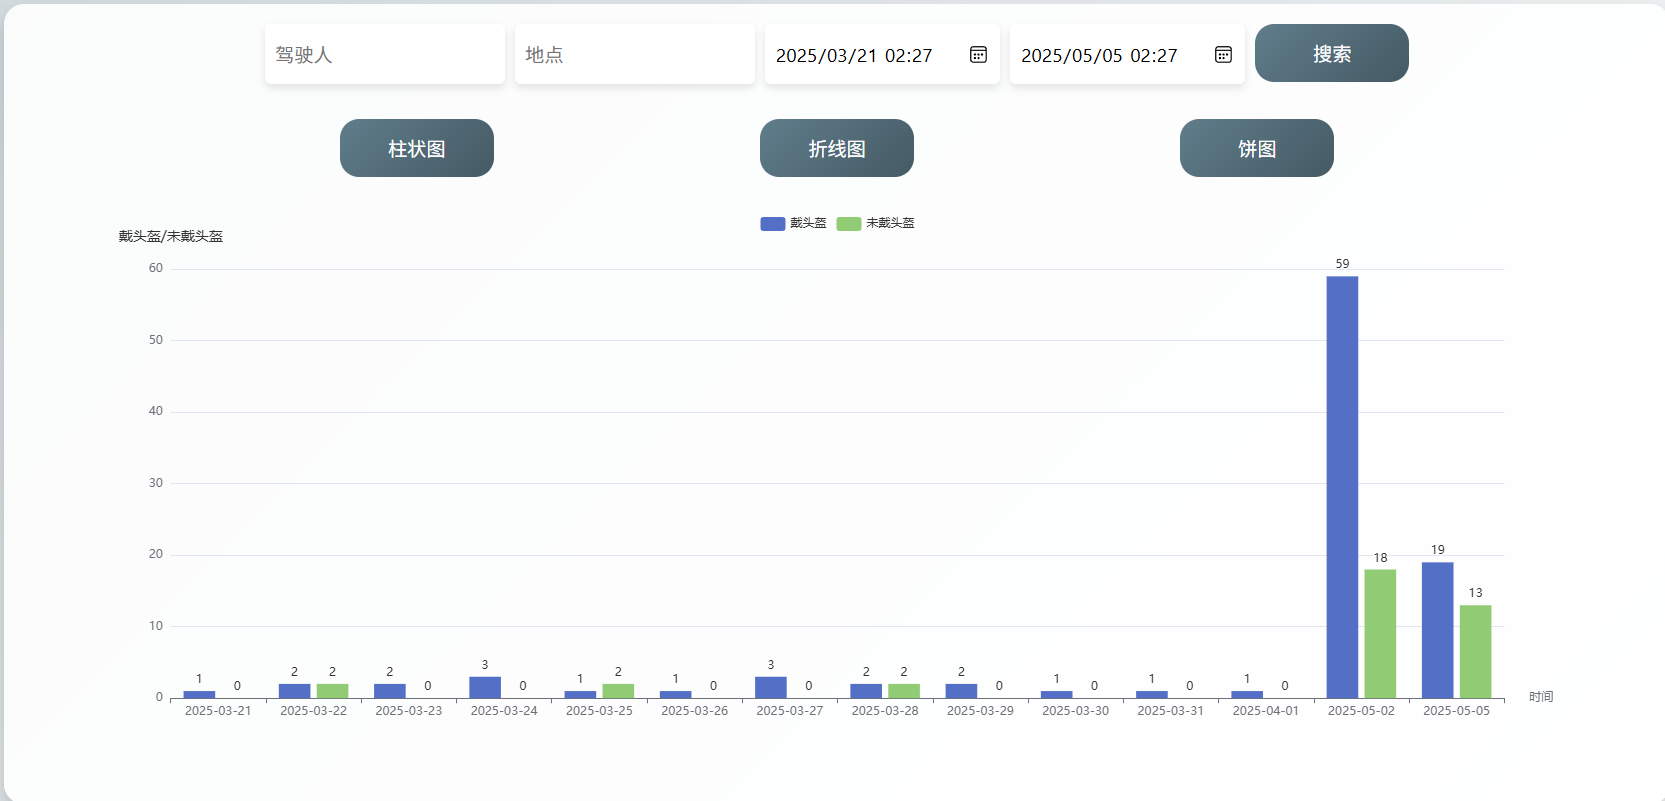
\includegraphics[width=\textwidth]{figs/chap05/data1.png}
        \caption{柱状图}
        \label{fig:data1}
    \end{minipage}
    \hfill % 使两张图片之间保持一定距离
    \begin{minipage}{0.3\textwidth}
        \centering
        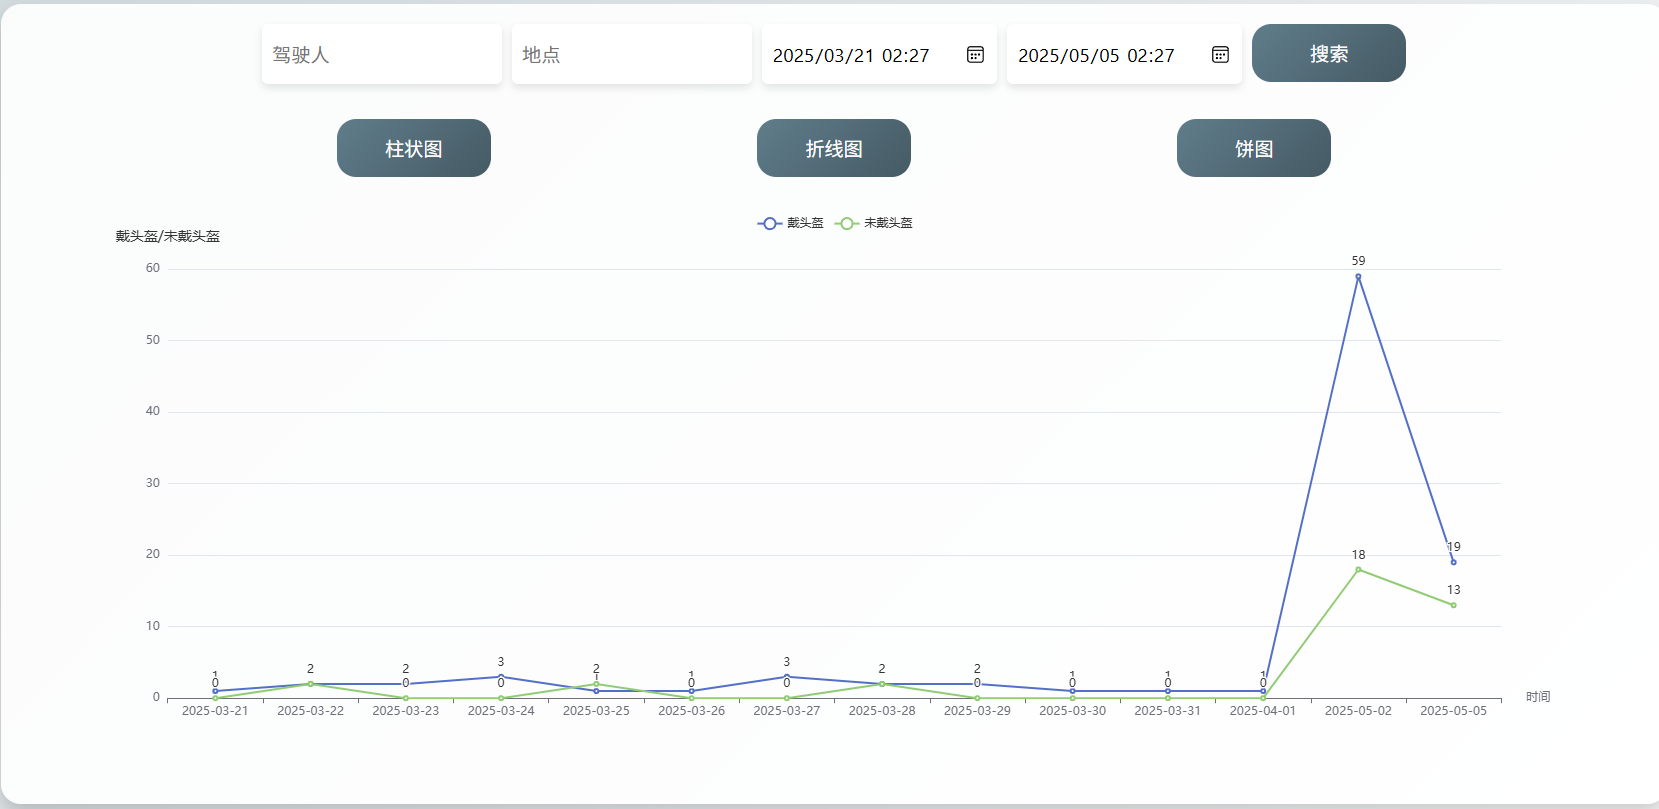
\includegraphics[width=\textwidth]{figs/chap05/data2.png}
        \caption{折线图}
        \label{fig:data2}
    \end{minipage}    
    \hfill % 使两张图片之间保持一定距离
    \begin{minipage}{0.3\textwidth}
        \centering
        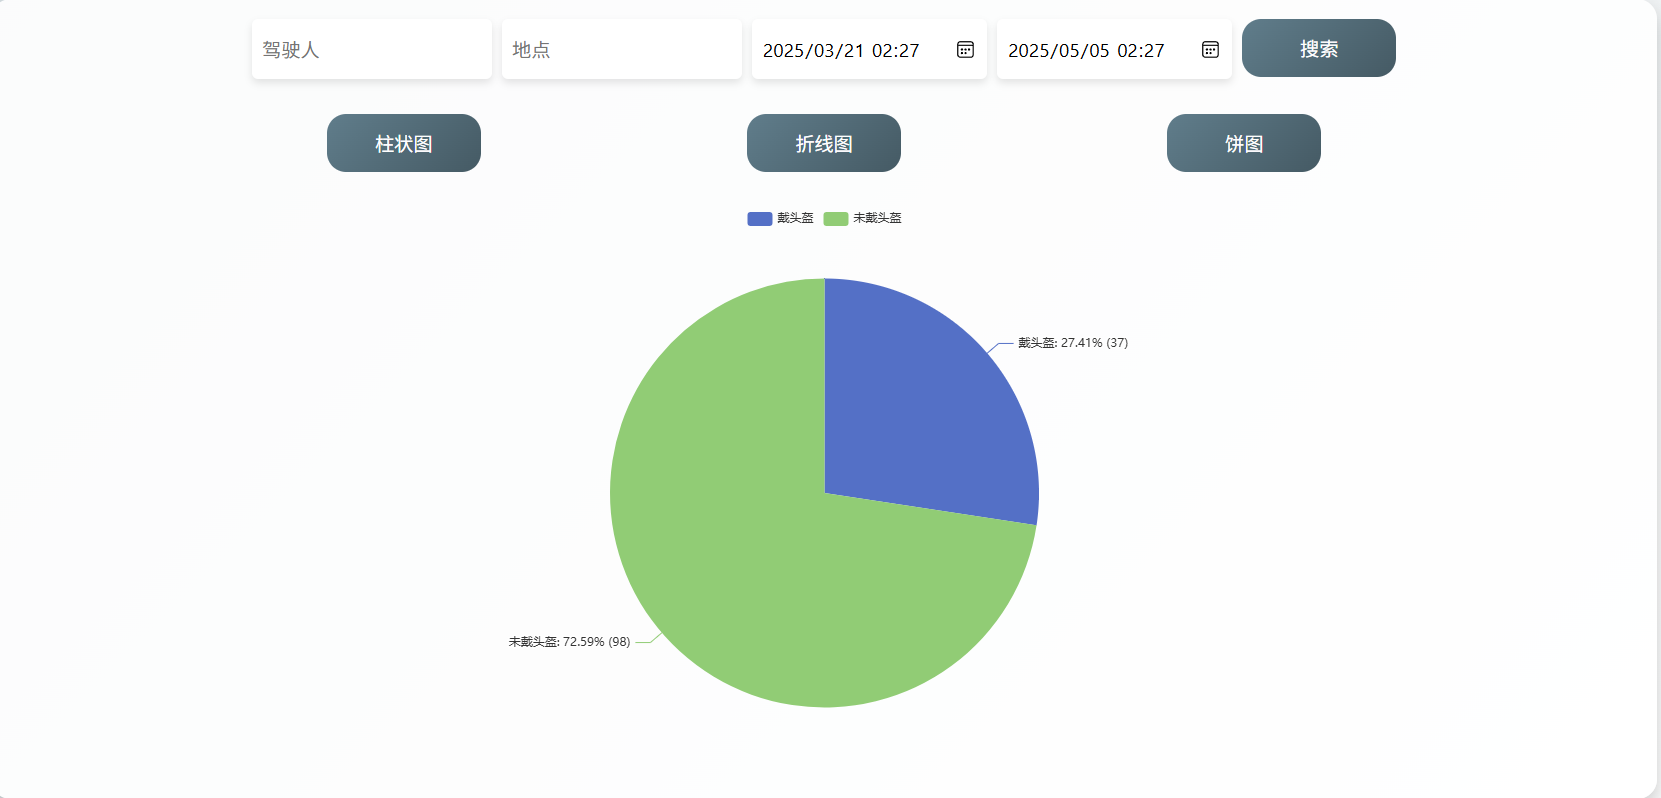
\includegraphics[width=\textwidth]{figs/chap05/data3.png}
        \caption{饼图}
        \label{fig:data3}
    \end{minipage}
  \end{figure}

\section{后端模块设计与实现}
由于Java语言强大的稳定性、跨平台性和丰富的第三方库,后端模块在框架上选用SpringBoot进行开发。为了便于系统的迭代和维护,在架构上选择MVC三层架构,即Controller层、Service层和Dao层。该系统主要分为两个模块:检测模块和搜索模块,负责实现前端页面提供的两大功能。

\subsection{库表结构}
该系统使用的库表结构如\ref{tab:datatable}所示。该表共有五个字段,除主键id外,记录了驾驶员信息、头盔佩戴情况、检测地区和检测时间。头盔佩戴情况在库表里面是以整型的方式记录的,节省空间且信息更加简洁,后端会对label和该字段的整型值做转换。由于在查询过程中,经常会对驾驶员信息和头盔佩戴情况这两个字段过滤,所以在设计的时候对这两个字段都创建了索引。

\begin{table}[htbp]
    \centering
    \caption{数据库表字段设计} % 表格标题,可根据实际情况修改
    \label{tab:datatable}
    \begin{tabular}{lccc} % l 表示左对齐,c 表示居中对齐,这里根据列数和对齐需求设置
        \toprule % 顶线
        字段 & 数据类型 & 说明 & 索引 \\
        \midrule % 中线
        id & int & 主键id & 主键索引 \\
        driver & varchar & 驾驶员 & 普通索引\\
        detect\_location & varchar & 检测地区 & 普通索引 \\
        helmet & int & 头盔佩戴情况 & 无 \\
        detect\_time & datetime & 检测时间 & 无 \\
        \bottomrule % 底线
    \end{tabular}
\end{table}

\subsection{检测模块}
该模块的执行流程图如\ref{fig:process1}所示,当接收到用户的检测请求时,首先会保存用户上传的原数据,然后会调用头盔检测模型检测数据中的头盔佩戴情况并保存检测结果到数据库。在检测驾驶员这一功能中,需要对原数据检测到的头盔佩戴目标框做裁剪,调用驾驶员检测模型检测每一个裁剪下来的小图片中的驾驶员,这个过程非常耗时,为了提高用户的使用体验,这里对驾驶员的检测会异步进行,不会阻塞用户的请求。YOLO模型对视频的预测结果默认为avi格式,avi格式的视频在目前各个浏览器上兼容性并不好且体积较大,所以后端这里会对视频检测结果做一个数据格式转换,由avi格式转换为兼容性更好的mp4格式。最后后端会构建好响应结果,返回数据给前端用户。

\begin{figure}[!htb]
    \centering
    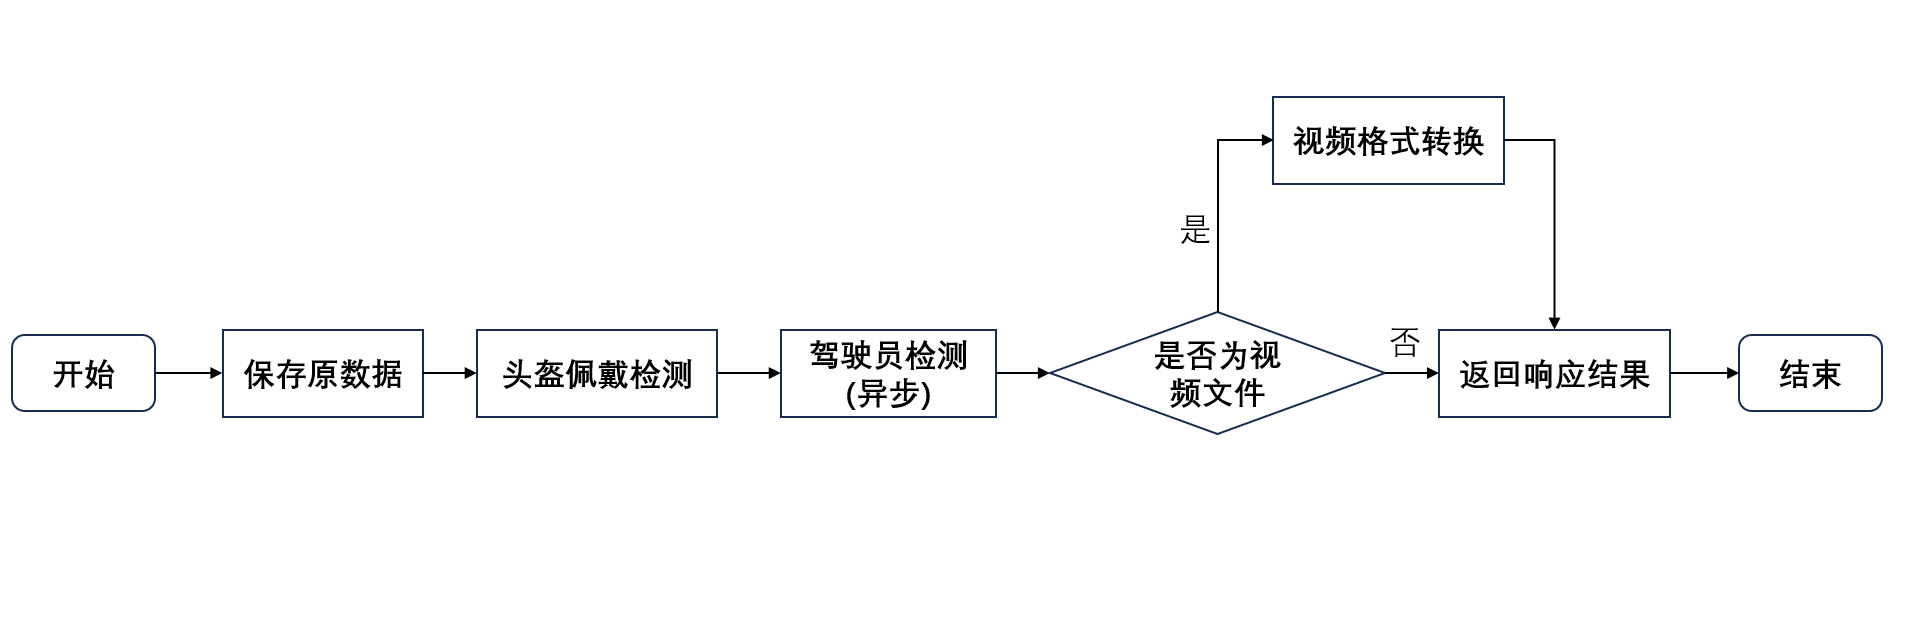
\includegraphics[width=0.9\textwidth]{figs/chap05/process1.png}
    \caption{检测模块执行流程}
    \label{fig:process1}
\end{figure}


\subsection{搜索模块}
该模块负责实现前端的记录查询功能,执行流程如\ref{fig:process2}所示。该模块会接收前端的搜索请求,并将过滤条件拼接到Sql语句中。如果前端传入的某一个字段过滤条件为空,则代表查询时不对该字段进行过滤。由于前端ECharts组件不同的可视化图标对数据的格式要求不同,还需要针对各个可视化图表的要求对数据作进一步处理。

\begin{figure}[!htb]
    \centering
    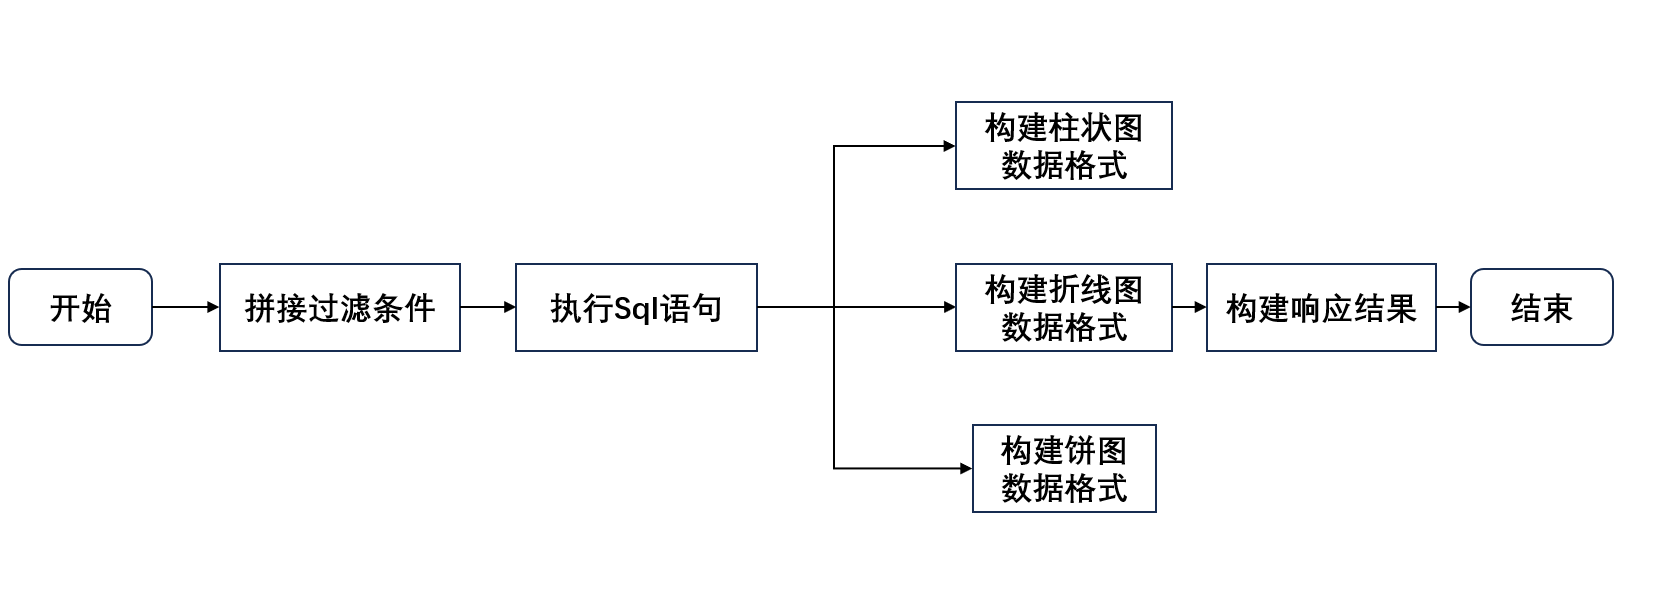
\includegraphics[width=0.9\textwidth]{figs/chap05/process2.png}
    \caption{搜索模块执行流程}
    \label{fig:process2}
\end{figure}

\section{本章小结}
本章详细介绍了基于Vue和SpringBoot框架的摩托车驾乘人员头盔佩戴检测系统的需求分析和界面实现。并对目标检测和结果查询两个前端页面的功能进行了测试。通过本章可知,该系统的前端和后端都已联通且功能正常。

% \chapter{多级标题}

% \section{演示一级标题}
% \subsection{演示二级标题}
% \subsubsection{演示三级标题}
% \subsubsection{再次演示三级标题}
% \subsection{另一个示二级标题}
% \subsubsection{另一个三级标题}
% \subsubsection{还有一个三级标题}

% \section{演示一级标题}
% \subsection{演示二级标题}
% \subsubsection{演示三级标题}
% \subsubsection{再次演示三级标题}
% \subsection{另一个示二级标题}
% \subsubsection{另一个三级标题}
% \subsubsection{还有一个三级标题}


%%% Local Variables: 
%%% mode: latex
%%% TeX-master: "../main.tex"
%%% End:
